   \section*{Instrukcje}
Będziesz mieć \textbf{\testDuration} minut na napisanie kodu,
który powinien przejść wszystkie
\textbf{\mycount} dostarczone testy. \\
Plik, w którym zapisane są wszystkie testy, nazywa się
\textbf{functions.test.js}.\\
Kod testów jest zahashowany, więc nie będziesz w stanie zrozumieć
jego szczegółów.\\

\begin{large}
	Wszystkie zadania muszą zostać zaimplementowane w JEDNYM i
	TYLKO JEDNYM pliku
	o dokładnej nazwie \textbf{functions.js}. Każda inna nazwa
	pliku nie zostanie
	zaakceptowana przez automatyczny system sprawdzający.
	
	Po zakończeniu implementacji plik \textbf{functions.js} musi zostać
	spakowany do archiwum o dokładnej nazwie \textbf{functions.zip},
	a następnie to archiwum musi zostać przesłane w ramach zadania.
	Nie akceptuję plików WORD, PDF ani żadnych innych nazw lub formatów.\\
	Musisz utworzyć plik \textbf{functions.js} i w tym pliku
	stworzyć oraz wyeksportować
	wszystkie funkcje/klasy wymagane przez testy, w następujący sposób:
\end{large}

\begin{minted}{javascript}
module.exports = {}
module.exports.example = example
\end{minted}

Oba te pliki muszą znajdować się w tym samym folderze — wymuszają to Jest i NPM.
\section*{Jak utworzyć środowisko do testowania} Wszystkie informacje zostały przedstawione na laboratoriach.

\begin{enumerate}
	\item Utwórz nowy, pusty folder,
	\item Pobierz archiwum z plikiem \textbf{\textit{functions.test.js}} z zadania na \textbf{MS Teams},
	\item Zainstaluj bibliotekę \textbf{\textit{\href{https://jestjs.io/docs/getting-started}{JEST}}}
	\begin{enumerate}
		\item Otwórz terminal / wiersz poleceń, przejdź do wcześniej utworzonego folderu i wykonaj polecenie: \\ \textbf{npm install --save-dev jest}
		\item W pliku \textit{package.json} dodaj:
	\end{enumerate}
\begin{minted}{javascript}
"scripts": {
	"test": "jest --noStackTrace --silent"
}
\end{minted}

	\item Aby sprawdzić, czy środowisko zostało poprawnie skonfigurowane, uruchom: \\ \textbf{npm run test}
\end{enumerate}

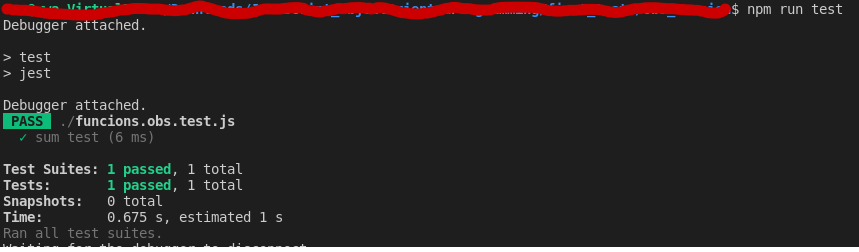
\includegraphics[width=\textwidth]{npm_run_test}
\subsection*{Zgodność z instrukcją}
Nazwy plików oraz wszystkie inne określone w instrukcji elementy muszą być dokładnie takie same.
W przeciwnym razie testy nie zostaną zaakceptowane.

\subsection*{Ocena}
Ocena obejmuje wyłącznie pliki znajdujące się w zasobie. Pliki te nie mogą być modyfikowane przez osobę sprawdzającą.
Każdy test, który przechodzi, daje 1 punkt, \textbf{pod warunkiem że program działa poprawnie jako całość}.

\begin{remarkbox}[title=Program działający]
	Za działający program uważa się taki, który poprawnie uruchamia się i kończy wykonanie, niezależnie od tego, czy wszystkie testy przechodzą.
	Program nie może wchodzić w nieskończone pętle ani zachowywać się w sposób nieoczekiwany (np. powodować błędów krytycznych lub awarii) ani zwracać sygnałów typu SIGTERM, SIGSEGV, SIGINT, SIGILL, SIGABRT, SIGFPE itp.
\end{remarkbox}

\subsection*{Dowód działania}
Screenshoty, printouty z konsoli ani inne materiały z własnych uruchomień nie są dowodem działania programu.
Kod jest uruchamiany przez osobę sprawdzającą i oceniany jest tylko wynik testu.

\subsection*{Zasady dotyczące zasobu}
Do swojego zasobu należy umieścić całe swoje rozwiązanie w formacie \textbf{zip} (\textit{projekt bez folderu node\_modules}).
Nazwa archiwum \textbf{nie może} zawierać znaków spoza UTF-8 ani znaków specjalnych (w tym spacji, nawiasów itp.).
Najlepiej, aby nazwa spakowanego projektu była taka sama jak archiwum udostępnione w zasobie. Inne formaty archiwum (rar, tar.*, .7z, .dmg ) nie beda sprawdzane.

\subsection*{Porządek w projekcie}
Z Twojego rozwiązania usuń folder \textbf{node\_modules} przed spakowaniem archiwum.